\chapter{Исследовательский раздел}
\section{Технические характеристики}
Технические характеристики устройства, на котором выполнялось тестирование:
\begin{itemize}
	\item операционная система: Windows 10 Pro;
	\item память: 8 Гб;
	\item процессор: Intel(R) Core(TM) i5-8265U CPU @ 1.60 ГГц   1.80 ГГц.
\end{itemize}
Тестирование проводилось на ноутбуке, который был подключен к сети питания. Во время проведения тестирования ноутбук был нагружен только встроенными приложениями окружения, самим окружением и системой тестирования.

\section{Сравнение алгоритмов}
Трудоемкость алгоритма оценивается по количеству сравнений, необходимых для поиска элемента. Размер массива, который был предварительно заполнен целыми числами случайным образом, составляет 1091. На рисунке~\ref{fig:Figure_1} представлена гистограмма, отражающая зависимость количества сравнений от индекса искомого элемента при линейном поиске.
\begin{figure}[H]
    \centering
    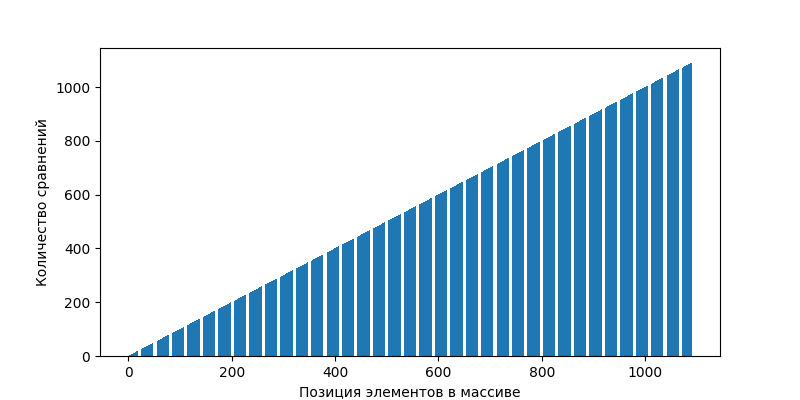
\includegraphics[width=1\textwidth]{images/Figure_1.png}
    \caption{Гистограмма зависимости числа сравнений от индекса искомого элемента при линейном поиске.}
    \label{fig:Figure_1}
\end{figure}

На рисунках~\ref{fig:Figure_2} и~\ref{fig:Figure_3} представлены гистограммы работы алгоритма бинарного поиска. Гистограмма на рисунке~\ref{fig:Figure_3} показывает количество сравнений, отсортированных по возрастанию.

\begin{figure}[H]
    \centering
    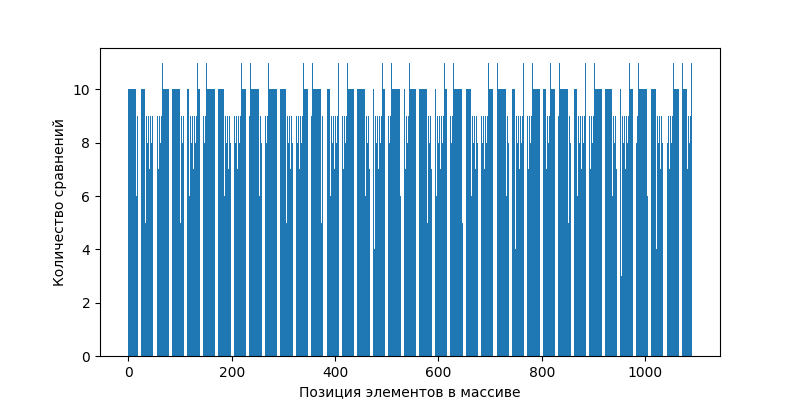
\includegraphics[width=1\textwidth]{images/Figure_2.png}
    \caption{Гистограмма зависимости числа сравнений от индекса искомого элемента при бинарном поиске.}
    \label{fig:Figure_2}
\end{figure}

\begin{figure}[H]
    \centering
    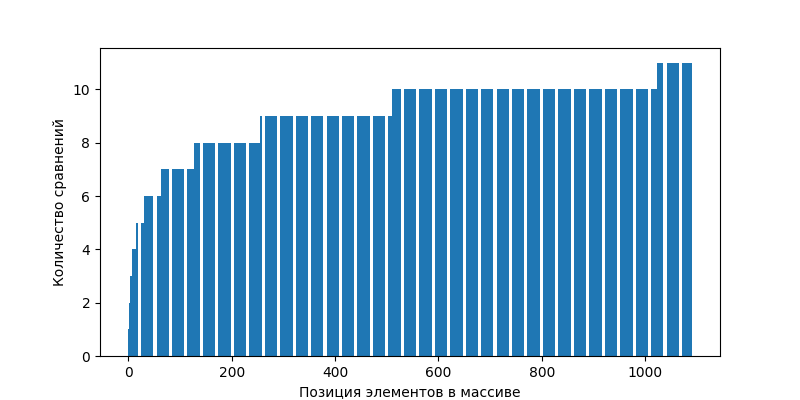
\includegraphics[width=1\textwidth]{images/Figure_3.png}
    \caption{Гистограмма зависимости числа сравнений от индекса искомого элемента при бинарном поиске, отсортированная по возрастанию количества сравнений.}
    \label{fig:Figure_3}
\end{figure}


\section*{Вывод}
В ходе исследования были рассмотрены и сравнены линейный и бинарный алгоритмы поиска. Линейный поиск выполняет последовательное сравнение элементов массива с искомым значением, что приводит к числу сравнений, равному позиции элемента плюс один. В худшем случае, если элемента нет в массиве, необходимо выполнить \( n \) сравнений, где \( n \)~---~размер массива. 

Бинарный поиск использует метод деления массива пополам, сокращая область поиска на каждом шаге. Это позволяет уменьшить количество сравнений: в худшем случае оно составляет примерно \( \log_2(n) \). Например, для массива из 50 элементов максимальное количество сравнений составит 6. Основное ограничение бинарного поиска заключается в необходимости предварительной сортировки массива, которая может потребовать дополнительных затрат времени.